\documentclass[a4paper]{report}
\usepackage[utf8]{inputenc}
\usepackage[utf8]{inputenc}
\usepackage[utf8]{inputenc}
\usepackage[utf8]{inputenc}
\usepackage[slovene]{babel}
\usepackage[euler]{textgreek}
\usepackage{xcolor}
\usepackage{cite}
\usepackage{graphicx}
\usepackage{subcaption}
\usepackage{natbib}
\usepackage{hyperref}
\usepackage{multicol}
\usepackage{float}
\usepackage{authblk}
\usepackage{caption}
\usepackage{ragged2e}
\usepackage{blindtext}
\DeclareGraphicsExtensions{{.jpg},{.png},{.pdf}}
%\doublespacing
%\usepackage{lipsum}
\usepackage{graphicx}
\begin{document}
\title{Vaja 15 Težno nihalo}
\author{Jure Kos }
\date{8.1.2022}
\graphicspath{{./images/} }
\maketitle


\chapter*{Uvod}
Nihajni čas matematičnega nihala (točkastega telesa na breztežni nitki), ki niha
nedušeno in z majhno amplitudo, je:

\[T=2\pi\sqrt{\frac{l}{g}}\]

Pri tej vaji želimo izračunati gravitacijski pospešek Zemlje. Pri tem uporabimo popravke, ki nam zgornjo formulo naredijo natančnejšo.\\
Tako dobimo natančnejšo formulo za g:

\[g = l_0(\frac{2\pi}{T})\cdot\Bigg[1+ \frac{1}{2}sin^2\frac{\alpha}{2}+\frac{2}{5}(\frac{r}{l_0})^2-1/6\frac{m_z}{m_k}+(1+k)\frac{\rho_{z_r}}{\rho_{F_e}}+(\frac{\Lambda}{2\pi})^2\Bigg]\]

\section*{Potrebščine}

1. Nihalo, obešeno na strop,\\
2. merilo z zrcalcem, pritrjenim na zidu,\\
3. vrvica,\\
4. štoparica,\\
5. kljunasto merilo,\\
6. vžigalnik.
\chapter*{Meritve}
\begin{figure}[H]
    \centering
    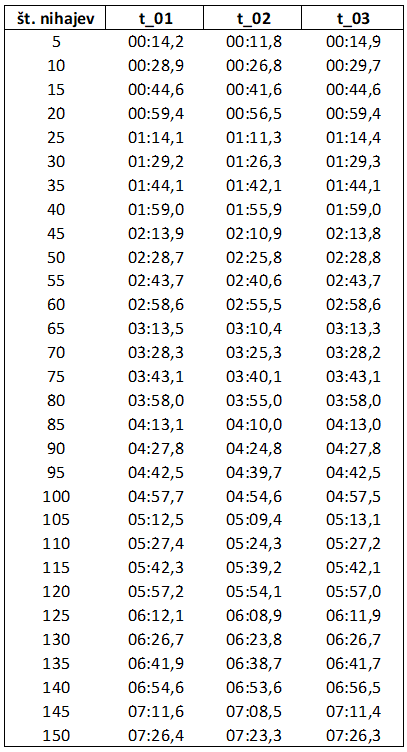
\includegraphics[scale=1]{Tabela meritev.png}
    \caption{Meritve nihajnih časov}
\end{figure}

l=210 cm $\pm$ 0,1 cm \\
a=4,3 cm $\pm$ 0.05 cm \\
h = 5,3 mm $\pm$ 0,01 mm\\
$r_z$=0,75 mm (1$\pm$ 0,013)\\
r = $\frac{-h^2-\frac{a^2}{3}}{-2h}$ = 6,07 cm (1$\pm$0,015)\\
$x_0$ = 20 cm \\
$x_{150}$ = 14,6 cm \\

\section*{Izračuni}
Izračun povprečnega nihajnega časa:\\
Najprej smo izračunali čase 5 nihajev za vsako vrstico meritev. To smo naredili tako, da smo odšteli čas v absolutnih enotah in s tem dobili časovno razliko. Tako smo naredili povprečje vseh meritev, ki je prišlo $ \overline{t_{5_{1}}} = 14,8675 s$ za prvo meritev in tako dobili povprečen nihajni čas enega nihaja prve meritve kot $\overline{{t_1}}$ = 2,9735 s (1 $\pm$ 0,00274). Seveda to ponovimo za vse 3 meritve in s tem lahko rezultate zapišemo v tabeli kot
\\
\begin{table}[H]
    \centering
    \begin{tabular}{c|c|c|c}
        Meritev &1&2&3  \\
        \hline
        Nihajni čas [s] &2,9735 &2.9414&2.9817\\
        Napaka [\%]& 0,269&0.2719&0.2683\\
    \end{tabular}
    \caption{Meritve nihajnih časov}
    \label{tab:my_label}
\end{table}
Iz vseh treh meritev lahko izračunamo povprečen čas $\overline{t}$, s katerim izračunamo pospešek kot 

\[ \overline{t} = \frac{t_1+t_2+t_3  }{3} = 2.9655 s (1\pm 0.00155)\]

Za uporabo zgoraj napisane formule potrebujemo izračunati še neznane količine. \\
Logaritemski dekrement izračunamo po formuli $ \Lambda=ln(\frac{x_n}{x_{n+1})},$ kjer je $x_n = x_0 e^{-\beta n T}$ amplituda n-tega nihaja. Izrazimo lahko $\beta$ kot

\[ \beta = -\frac{ln(\frac{x_n}{x_0})}{nT}\] [n=150] {$x_n$ in $x_0$ poznamo}

\[\beta = 5,021 \cdot 10^{-4}\cdot(1 \pm0,03)\]

Izračunamo dalje 

\[ \Lambda = ln\frac{x_0e^{-\beta nT}}{x_0e^{-\beta (n+1)T}}= T\beta = 1.488\cdot10^{-3} (1\pm0,039)\]

Izračunajmo še odklon nihala. Tega dobimo kot

\[ sin \alpha = \frac{x_0}{l} \longrightarrow \alpha=arcsin(\frac{x_0}{l}) = 5,46^\circ \]

Za izračun potrebujemo le še masi krogle in žice

\[ m_k = \frac{4\pi r^3}{3}\rho_{F_e} = 7,3 kg (1\pm0,03)
\]

 \[m_z = \pi r_z^2 l_0 \rho_{jeklo} = 0,0308 kg(1\pm0,026) 
\]

\section*{Izračun gravitacijskega pospeška}

Zdaj lahko vstavimo vse številke v formulo za gravitacijski pospešek in dobimo

\[g = 9,80624 \frac{m}{s^2}\]

Po izračunu napake dobimo

\[\Delta g  = 2,3\cdot 10^{-3} \frac{m}{s^2}\]
%= (\Delta_{l_0} + 2 \Delta_T)\frac{2/5 r^2/l_0(2 \Delta_{l_0+2} \Delta_r)+\frac{m_z}{6m_k}( \Delta_m+ \Delta_z)+(\Lambda/2\pi)^2(2 \Delta_\Lambda+ \Delta_{sin\alpha}}{1+1/2 sin\alpha/2 + 2/5 r^2/l_0 - \frac{m_z}{6m_k} + (1+k)\frac{\rho_z}{\rho_{F_e}} + (\Lambda/2\pi)^2}

Dobimo končno vrednost:\\

\[g= 9,80624 \frac{m}{s^2} \pm 2,3\cdot 10^{-3} \frac{m}{s^2} = 9,80624 \frac{m}{s^2} (1\pm 0,000235)\]

Za primerjavo lahko izračunamo pospešek z uporabo formule za matematično nihalo 

\[ g=l_0 (\frac{2\pi}{T}) = 9,856 (1\pm 0,0059) \frac{m}{s^2}\]

\end{document}


